\documentclass[11pt]{article}
\usepackage[letterpaper,margin=0.72in]{geometry}
\usepackage{graphicx,tabularx,booktabs,array,xcolor,hyperref,longtable,multicol}
\usepackage[T1]{fontenc}
\usepackage{lmodern}
\definecolor{acpink}{HTML}{C04486}
\definecolor{acgray}{HTML}{55515A}
\definecolor{acpaper}{HTML}{FFF9FC}
\hypersetup{colorlinks=true,urlcolor=acpink,linkcolor=acpink}
\setlength{\parindent}{0pt}
\setlength{\parskip}{0.55em}
\newcommand{\ac}{\textcolor{acpink}{Aesthetic Computer}}
\newcommand{\mediumtitle}[1]{\section*{\Huge\color{acpink}#1}}
\begin{document}

{\Huge\bfseries\color{acpink} Audio You Can Hand Someone}\par
{\Large A physical-media catalog for \ac{} podcasts and /pop}\par
\textcolor{acgray}{Prepared July 18, 2026 · cassette, vinyl, CD, and audiovisual appendix}

\vfill
\begin{center}
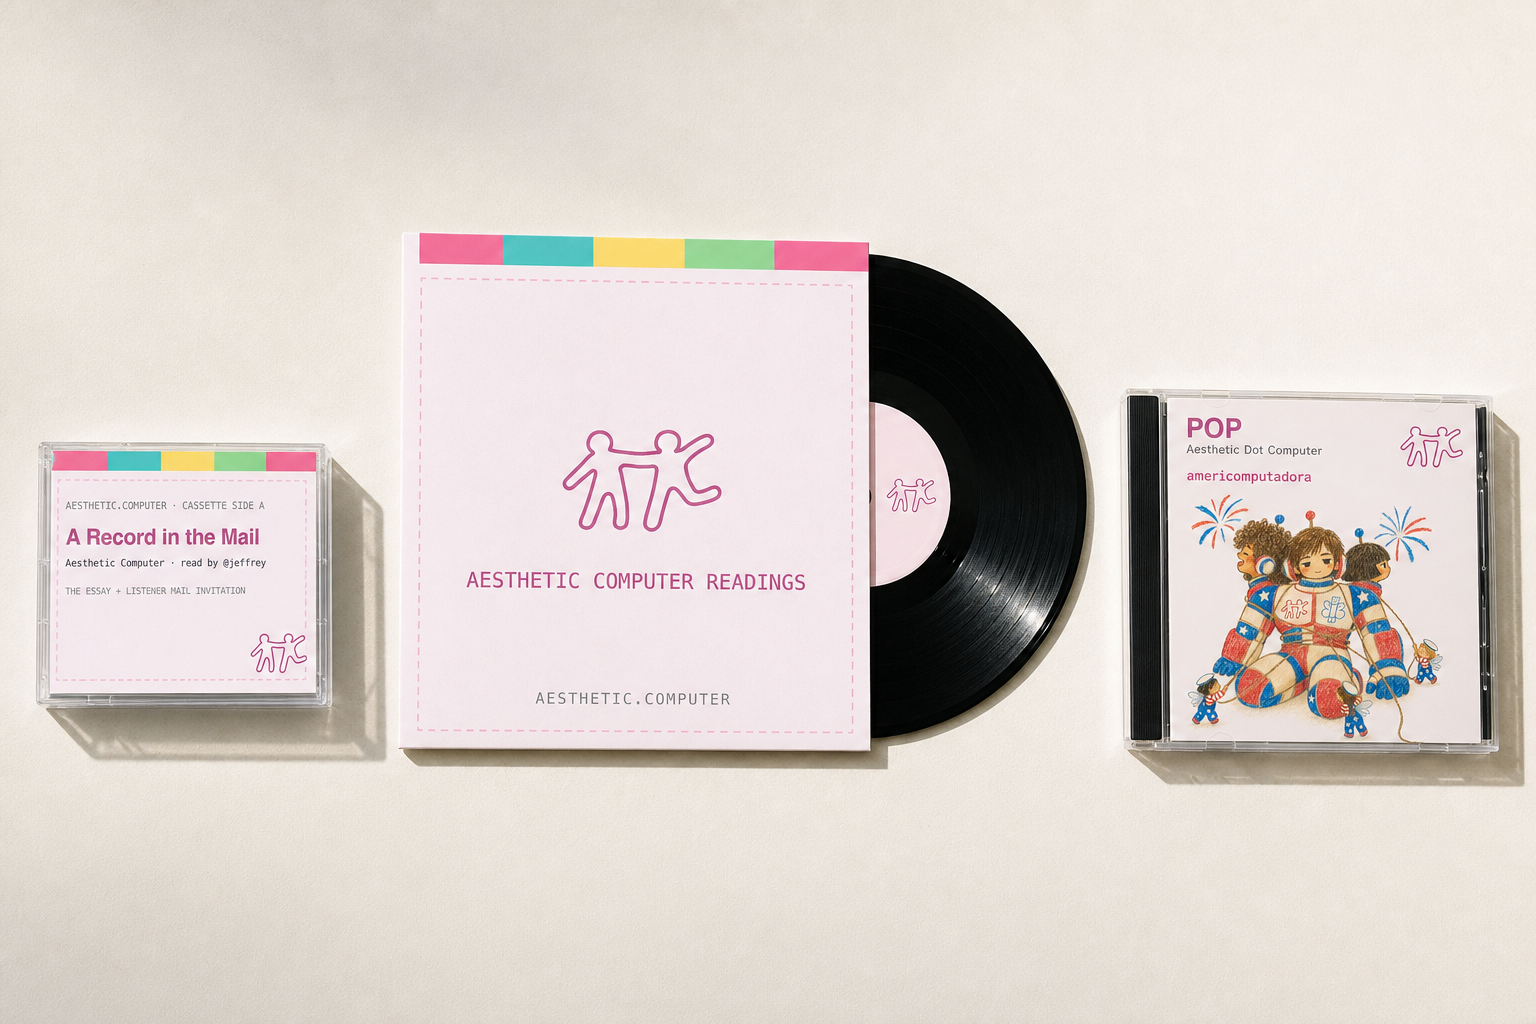
\includegraphics[width=\textwidth]{ac-physical-media-cross-section.png}
\end{center}
\vfill

\textit{A showable concept catalog backed by current Kunaki specifications, live shipping quotes, and production-ready podcast masters. The photographed products are mockups; no physical order has been placed.}

\clearpage
\section*{The proposition}

\ac{} already makes two complementary kinds of audio. The podcast turns essays and technical sessions into spoken objects: a voice carries an argument into a car, a room, or a walk. The \texttt{/pop} studio makes rendered songs, procedural tracks, long-form systems, and families of variations. Both begin as files. Physical media gives those files scale, sequence, weight, edges, and a reason to be passed from one person to another.

This catalog is designed to be shown to a collaborator, label, shop, listener, or potential patron. It asks a simple question: \emph{which object should this sound become?}

\begin{tabularx}{\textwidth}{>{\bfseries}l X X r}
\toprule
Medium & What it communicates & Strongest AC use & Proof delivered* \\
\midrule
Cassette & intimate, handmade, serial & podcast episodes; variant families & \$10.72 \\
CD jacket & inexpensive, complete, mailable & /pop compilations; podcast season & \$7.22 \\
12-inch vinyl & editioned, ceremonial, displayable & selected readings; focused album & \$46.71 \\
7-inch vinyl & single, artifact, concise statement & short /pop single with B-side & quote at checkout \\
DVD/Blu-ray & audio joined to moving image & visual albums; software/video editions & appendix \\
\bottomrule
\end{tabularx}

{\small *Manufacturing plus the least expensive live shipping quote to ZIP 90012, using Kunaki's public sample product for that medium. Final products must be re-quoted. Taxes are not included.}

\section*{The source collection}

\textbf{Published podcast:} three episodes, 32 minutes 58 seconds total. Each episode has a finished MP3, upload-ready cassette WAV, label art, J-card art, and a manifest.

\textbf{/pop library:} 106 indexed renders spanning released, mastering, work-in-progress, and unreleased states. This report deliberately samples finished works and coherent variant families instead of pretending every render is a release.

\textbf{Representative released works:} \textit{americomputadora} (2:29), \textit{fluttabap360} (6:00), \textit{momabobasheep} (10:00), \textit{amaythingra} (4:33), \textit{marimbaba} (1:24), and \textit{helpabeach} (2:31).

\textbf{Representative edition families:} \textit{cutezen / cutezip / cutezenith} (6:54 combined) and four \textit{cornerfive} mixes (5:36 combined). These are especially well suited to cassette sides or a short CD because physical sequencing turns revisions into a legible work.

\clearpage
\mediumtitle{Cassette}

\begin{center}
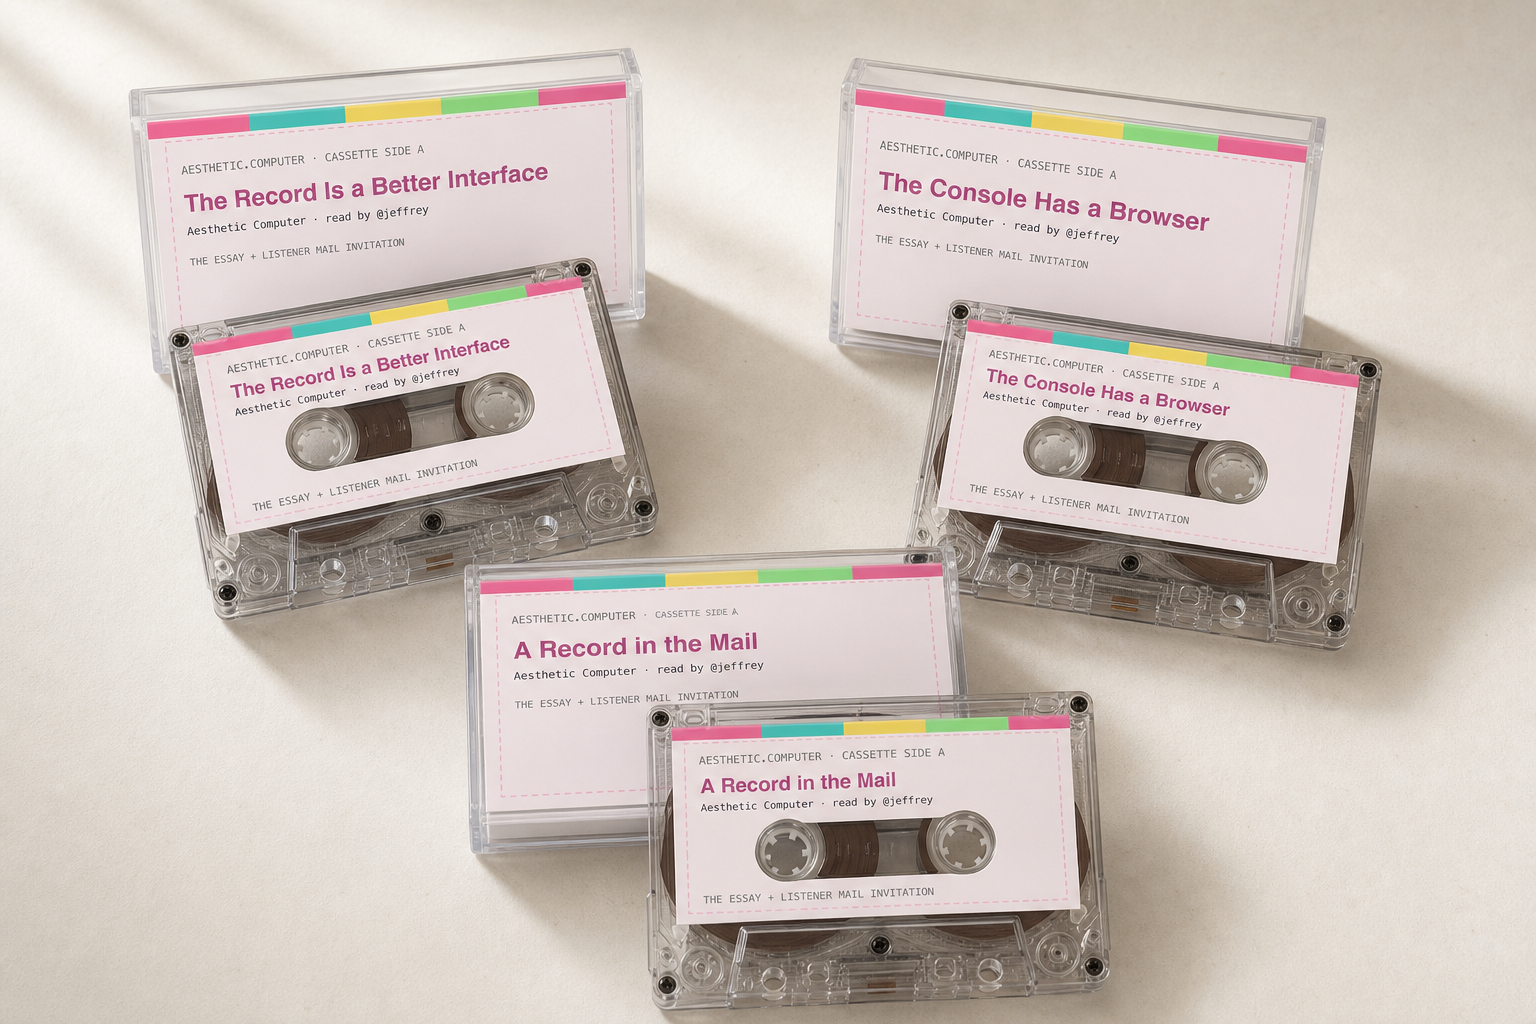
\includegraphics[width=\textwidth]{ac-podcast-cassette-collection.png}
\end{center}

Cassette is the strongest first object for the podcast. It is inexpensive enough to proof without ceremony, culturally comfortable with spoken word, and mechanically supplies an intermission: Side A ends, the listener turns the tape, and Side B can answer it.

\subsection*{Podcast edition}

\begin{tabularx}{\textwidth}{>{\bfseries}X r r X}
\toprule
Episode & Runtime & Side used & Proposed Side B \\
\midrule
The Record Is a Better Interface & 9:28 & 24\% & controller sounds; tactile appendix \\
The Console Has a Browser & 13:05 & 33\% & Xbox field notes; gamepad sonification \\
A Record in the Mail & 10:25 & 26\% & listener letters; sources; reply \\
\bottomrule
\end{tabularx}

All three can also fit together on a single tape: two episodes on Side A and one episode plus correspondence on Side B. Separate tapes, however, make the titles showable and let each episode remain open to a changing B-side.

\subsection*{/pop cassette proposals}

\begin{itemize}
  \item \textbf{Cutezen Variations:} \textit{cutezen}, \textit{cutezip}, and \textit{cutezenith} on Side A; sketches or alternate engine renders on Side B.
  \item \textbf{Cornerfive: Four Corners:} original, dub, footwork, and music-box versions as one deliberately sequenced object.
  \item \textbf{Long Systems:} \textit{momabobasheep} and \textit{fluttabap360} paired across sides, allowing procedural duration to remain audible.
  \item \textbf{Letters and Signals:} a hybrid tape of a podcast reading, gamepad tones, environmental captures, and listener correspondence.
\end{itemize}

\subsection*{Kunaki cassette specification}

90-minute stereo cassette; 40-minute maximum per side; full-color labels and case insert. Artwork is JPEG at 300 DPI with no bleed: J-card 1200 $\times$ 1110 pixels, each rectangular label 1062 $\times$ 496 pixels. Kunaki accepts WAV, MP3, AAC, WMV, and M4A. The published manufacturing price is \$5.00 each for quantities 1--999.

\textbf{Live proof estimate to Los Angeles:} \$5.00 manufacture + \$5.72 USPS First Class (2--5 business days) = \textbf{\$10.72 delivered before tax}.

\clearpage
\mediumtitle{12-inch Vinyl}

Vinyl is not the economical default. It is the edition that says a particular recording deserves a front, a back, a large image, and twenty uninterrupted minutes per side. It is best used selectively: one foundational reading, one concentrated /pop album, or a deliberately paired argument and response.

\subsection*{Podcast fit}

Every current episode fits on one 20-minute side. Three useful configurations follow:

\begin{enumerate}
  \item \textbf{One essay / one response:} reading on Side A; sources, letter, or newly recorded answer on Side B.
  \item \textbf{Two-episode pairing:} \textit{The Record Is a Better Interface} and \textit{The Console Has a Browser} as material interface / console interface.
  \item \textbf{The mail object:} \textit{A Record in the Mail} on Side A and the sound of making and receiving its first proof on Side B.
\end{enumerate}

The entire three-episode catalog is 32:58 and therefore fits across a 40-minute two-sided record, leaving roughly seven minutes for an introduction, locked-groove-like ambience, or a brief letter. Kunaki's standard product is cut as a single 12-inch record; it cannot package multiple discs in one jacket.

\subsection*{/pop vinyl proposals}

\textbf{Aesthetic Dot Computer: Six Works} can place the six representative released tracks across two sides for approximately 27 minutes total. A tighter LP would choose four tracks and preserve more groove width. A focused conceptual record could instead pair \textit{momabobasheep} with \textit{fluttabap360} and supporting short pieces.

The strongest visual candidate is \textit{americomputadora}: it already has distinctive cover art, a concise runtime, and an identity that can anchor a compilation. As a 7-inch single it requires a B-side; as a 12-inch it should join a larger program.

\subsection*{Kunaki vinyl specification}

Standard product: black 12-inch, 180-gram stereo vinyl, 20 minutes maximum per side, full-color center labels, inner sleeve, full-color jacket, and cellophane wrap. JPEG/RGB artwork is printed at 300 DPI with no bleed. Jacket: 3675 $\times$ 3675 pixels. Labels: 990 $\times$ 990 pixels. Published price: \$36.00 per black record; picture or colored vinyl: \$50.00. A black 7-inch record is \$15.00 and holds seven minutes per side.

\textbf{Live 12-inch proof estimate to Los Angeles:} \$36.00 manufacture + \$10.71 USPS Media Mail (6--21 business days) = \textbf{\$46.71 delivered before tax}. UPS Ground raises the delivered proof to \$56.78 but advertises 1--5 business days.

\clearpage
\mediumtitle{Compact Disc}

CD is the most efficient catalog object. It holds 80 minutes of audio, carries enough print area to explain a project, costs less than a cassette, and is simple to mail. It is less romantic, but that restraint is useful: CD can become the complete sampler handed to someone after a meeting.

\subsection*{Podcast season disc}

All three podcast episodes occupy 32:58, leaving about 47 minutes. A first-season disc can include spoken introductions, source notes, listener letters, short pieces from \texttt{/pop}, or data files if created as a mixed/data-oriented edition. Kunaki offers only a two-panel insert in its jewel case, so a QR code to the living papers index should carry deeper notes.

\subsection*{/pop sampler disc}

A client-facing CD could gather the six representative released works, followed by the Cutezen and Cornerfive families. This makes the disc both album and evidence: finished distribution-ready songs first, then procedural variants demonstrating how the studio thinks.

Suggested sequence:

\begin{multicols}{2}
\begin{enumerate}
  \item americomputadora
  \item amaythingra
  \item helpabeach
  \item marimbaba
  \item fluttabap360
  \item momabobasheep
  \item cutezen
  \item cutezip
  \item cutezenith
  \item cornerfive
  \item cornerfive-dub
  \item cornerfive-footwork
  \item cornerfive-musicbox
\end{enumerate}
\end{multicols}

\subsection*{Kunaki CD specification}

Audio CD capacity is 80 minutes or 700 MB. Audio uploads accept WAV, MP3, AAC, WMV, or M4A; Kunaki masters them and inserts two-second track gaps. Artwork is JPEG/RGB, 300 DPI, no bleed. Disc art is a 1394-pixel square. Jewel case front and insert are 1423 $\times$ 1411; tray card is 1772 $\times$ 1385. The wraparound jacket is 3000 $\times$ 1500.

Published prices: \$2.00 jewel case, \$1.50 printed jacket, or \$0.75 disc only. All have a one-unit minimum.

\textbf{Live jacket-CD proof estimate to Los Angeles:} \$1.50 manufacture + \$5.72 USPS First Class = \textbf{\$7.22 delivered before tax}. A jewel-case proof is approximately \textbf{\$7.72}. This is the recommended show-and-tell sampler.

\clearpage
\mediumtitle{7-inch, Picture Vinyl, and Color Vinyl}

These are not merely price variants. Each changes what kind of claim the work makes.

\textbf{7-inch black vinyl --- \$15.00:} seven minutes per side. Best for a short /pop single plus a true B-side. \textit{americomputadora}, \textit{amaythingra}, or \textit{helpabeach} fit easily. None of the podcast episodes fits on one side without splitting or editing, so it is not recommended for the current readings.

\textbf{12-inch picture vinyl --- \$50.00:} an image is placed beneath the grooves on both sides. Best when the picture is part of the work, not merely decoration. The strong \textit{americomputadora} artwork makes it a plausible edition, but sound and print should be proofed before promising fidelity.

\textbf{12-inch color vinyl --- \$50.00:} supports a color choice while retaining the standard full jacket. The AC magenta/cyan/yellow/mint palette could become a series in which medium color indexes a family of recordings.

\textbf{Display-only vinyl --- \$11.00:} Kunaki also advertises black or picture records without grooves or audio. These are props or visual artifacts, not playable editions. They could be useful for an exhibition mockup, but should never be represented as records.

\section*{Which object to show whom}

\begin{tabularx}{\textwidth}{>{\bfseries}l X X}
\toprule
Person & Hand them & Why \\
\midrule
Listener / correspondent & one podcast cassette & intimate; directly invites a reply \\
Label / music collaborator & /pop jacket CD & broadest evidence at lowest cost \\
Curator / collector & one focused vinyl proof & large visual field and edition logic \\
Developer / platform partner & CD plus API manifest & demonstrates catalog and fulfillment together \\
Press / event visitor & cassette or 7-inch single & memorable, concise, easy to explain \\
\bottomrule
\end{tabularx}

\clearpage
\mediumtitle{DVD and Blu-ray Appendix}

Kunaki also supports DVD and Blu-ray duplication, cases, printed discs, one-unit manufacturing, direct shipment, and the same family of XML/HTTP/manual fulfillment interfaces. These become relevant when the sound is inseparable from moving image.

The \texttt{/pop} tree already contains such candidates. \textit{amaythingra} has reel and story video outputs. \textit{sineabye} has rendered path-traced, raster, CUDA, spin, and telemetry videos. A visual album or software-process edition could place the finished film in a standard player format and include source notes or alternate renders as data.

DVD/Blu-ray should not be used merely because they are available. They make sense when the screen is part of the score: a rendered world, performance capture, visualizer, console session, or documentary of the system producing the sound. Current price and exact case configuration should be pulled at product creation because this report's proof budget focuses on the three audio-native formats.

\section*{Fulfillment and API}

Across the product pages, Kunaki advertises one-unit manufacturing, direct drop-shipping, manual and CSV fulfillment, sales pages, and XML/HTTP interfaces. The endpoint has been verified with non-destructive shipping requests for public cassette, CD, and vinyl samples.

The API begins \emph{after} publication. New titles must be created in Kunaki's browser uploader. Audio and artwork are reviewed in a virtual player, then Kunaki issues a ten-character product ID. Our local client can use that ID to request shipping options, construct test orders, place explicitly authorized live orders, and retrieve status or tracking. Live order construction is blocked unless \texttt{KUNAKI\_ALLOW\_LIVE=1} is intentionally set.

Product pages say inactive titles may be deleted after 180 days without a purchase. A durable catalog therefore needs a small maintenance schedule or a reproducible release manifest that can recreate a removed title.

\clearpage
\section*{Proof budget and buying sequence}

\begin{tabularx}{\textwidth}{>{\bfseries}X r r r}
\toprule
Proof & Manufacture & Live economy shipping* & Delivered* \\
\midrule
A Record in the Mail cassette & \$5.00 & \$5.72 & \$10.72 \\
/pop sampler, jacket CD & \$1.50 & \$5.72 & \$7.22 \\
Aesthetic Computer Readings, black 12-inch & \$36.00 & \$10.71 & \$46.71 \\
\midrule
One of each medium & \$42.50 & \$22.15 & \textbf{\$64.65} \\
\bottomrule
\end{tabularx}

{\small *Quotes retrieved July 18, 2026 for ZIP 90012 using public sample IDs. The three products were quoted separately. A combined real order may change shipping. Taxes and payment-processing costs are excluded.}

\textbf{Stage 1 --- \$10.72 target:} publish and order \textit{A Record in the Mail} on cassette. Check audio level, stereo balance, hiss, label/window interaction, print color, J-card folds, case fit, packing, and actual transit time.

\textbf{Stage 2 --- \$7.22 target:} build one \texttt{/pop} jacket CD as the broad show-and-tell sampler. Confirm track gaps, metadata, disc printing, and whether the jacket feels substantial enough; upgrade to the \$2 jewel case if the spine and tray card matter.

\textbf{Stage 3 --- \$46.71 target:} only after the low-cost proofs pass, cut one black 12-inch. Choose either the three-reading collection or a focused /pop program. Check surface noise, level, track boundaries, label centering, jacket crop, seam strength, and cellophane.

\textbf{Stage 4:} photograph the received objects beside the mockups, revise the templates, assign retail prices, and expose only products that passed physical inspection.

\section*{Recommendation}

The best catalog is not every file on every medium. It is a small grammar:

\begin{itemize}
  \item \textbf{Cassette means correspondence.} One reading, one response, a changing Side B.
  \item \textbf{CD means catalog.} Many tracks, low cost, something complete to hand a person.
  \item \textbf{Vinyl means edition.} A selected work with enough visual and conceptual weight to justify the object.
  \item \textbf{DVD/Blu-ray means audiovisual score.} Sound whose moving image is not optional.
\end{itemize}

Begin with cassette and CD for \textbf{\$17.94 estimated delivered total if ordered separately}. They test nearly the whole pipeline for less than half the cost of the vinyl alone. Then make the record as the culmination, not the experiment.

Questions and feedback can go to \href{mailto:mail@aesthetic.computer}{mail@aesthetic.computer}. Unless the writer asks otherwise, their letter may be read or mentioned on a future episode---and, fittingly, may become part of a future Side B.

\vfill
\textcolor{acgray}{Mockups: built-in OpenAI image generation using exact AC artwork as references. Production data: Kunaki product and fulfillment pages checked July 18, 2026; local \texttt{/pop} library index; finished podcast masters. No purchase or charge was made.}

\end{document}
